\documentclass{article}
\usepackage[utf8]{inputenc}
\usepackage{amsmath}
\usepackage{amssymb}
\usepackage{graphicx}
\usepackage[english]{babel}
\usepackage{amsfonts}
\usepackage{fancyvrb}
\usepackage{xcolor}
\usepackage{listings}
\usepackage{graphicx}
\usepackage{mathrsfs}
\usepackage[margin=60pt, footskip=20pt]{geometry}
\definecolor{MyDarkGreen}{rgb}{0.0,0.4,0.08}
\usepackage{tabularx}
\usepackage{blindtext}
\usepackage{wrapfig}

\begin{document}
	
\pagenumbering{gobble}
\vspace*{-1.5cm}{
	\begin{center}
		\large
		POLITECNICO DI MILANO\\
		\normalsize
		Master Degree in Mathematical Engineering\\
		Industrial and Information Engineering\\
		Department of Mathematics\\
		\begin{figure}[htbp]
			\begin{center}
				
\includegraphics[width=3.5cm]{polimi.jpg}
			\end{center}
		\end{figure}
		\vspace*{0.3cm} \LARGE
		
		
		
		\textbf{Air Quality forecasting}\\
		
		
		\vspace*{.75truecm}\large
		\vspace*{.5truecm} \large
		 Bayesian Statistics Project Report
	\end{center}
	\vspace*{3.0cm} \large

	\begin{flushright}
		
		
		Group members:\\
		Datena Maria Alfredo \\
		Dell'Atti Martina \\
		Palummo Alessandro
		
		
	\end{flushright}
	\vspace*{2.0cm}
	\begin{center}
		
		
		
		Academic Year 2020-2021
	\end{center} \clearpage
}

\section{Wiseair and data measurement}

\subsection{Wiseair}

The measure of air quality in Lombardy is carried out by ARPA using accurate sensing stations. These stations, however, are expensive and bulky, so only a few of them are deployed on the territory. Only two of these stations are present in Milan. 

The concentration of particulate matter (PM), however, varies at an hyperlocal scale, so 2 stations are not enough to capture the phenomenon. 

Wiseair is a startup company that has designed a low-cost sensor, meant to be user-friendly and easy to install: Arianna. More than 100 citizens preordered one, and 50 of these sensors have been distributed in July 2020, thanks to the involvement of citizens.

\subsection{Objective}

Wiseair's goal is to provide citizens with useful information about air quality. To achieve this, the information coming from the Ariannas needs to be interpolated on areas where sensors are not present. Also, an air quality forecast would be useful, for example for planning outdoor activities. 

\subsection{Data measurement}

An Arianna sensor measures the concentration of PM once per hour or more frequently. The sensor also measures humidity and temperature with each PM measurement. It has been observed that the measurement accuracy is negatively affected by adverse weather conditions, so raw data can be filtered and processed so that outliers can be detected and removed, also using humidity and temperature information.

\section{Database structure}

Each observation in the dataset is a measurement from and Arianna station. 
The variable "PotID" identifies which sensor has taken the measurement. The ID is useful to geolocalize the measurement.
The variable "created\_at" gives the time coordinate for the measurement, up to the second. The format is "yyyy-mm-dd hh:MM:ss".
There are 6 variables related to air quality measurement, one for each of the following particulate matter types: PM_{1},PM_{2.5},PM_{10}. These types refer to the thickness of the measured particulate (for example, the variable PM{2.5} refers to particles of less than 2.5 micrometers


------
Originally we had data with a non regular frequency, i.e. the frequency of measurements of a sensor 
is different from others. For example, some pot-id make two measurements for hour, other pot-id make 
five measurements for hour. So we have performed an hourly average of the measured quantities in order to have equally spaced points. We choose to aggregate hourly because of two reasons: 
\begin{itemize}
\item This choice does not remove eventual patterns during the day, differently from the case in which we tried to aggregate taking daily averages. 
\item Weather data (rain level, wind speed) from ARPA are available with hourly frequency so we needed to average 
available data hourly before integrating further information from ARPA sensors. 
\end{itemize}

------
\newpage
\section{\textbf{Univariate Analysis}}
\subsection{Exploration analysis}
\begin{figure}[h!]
    \centering
    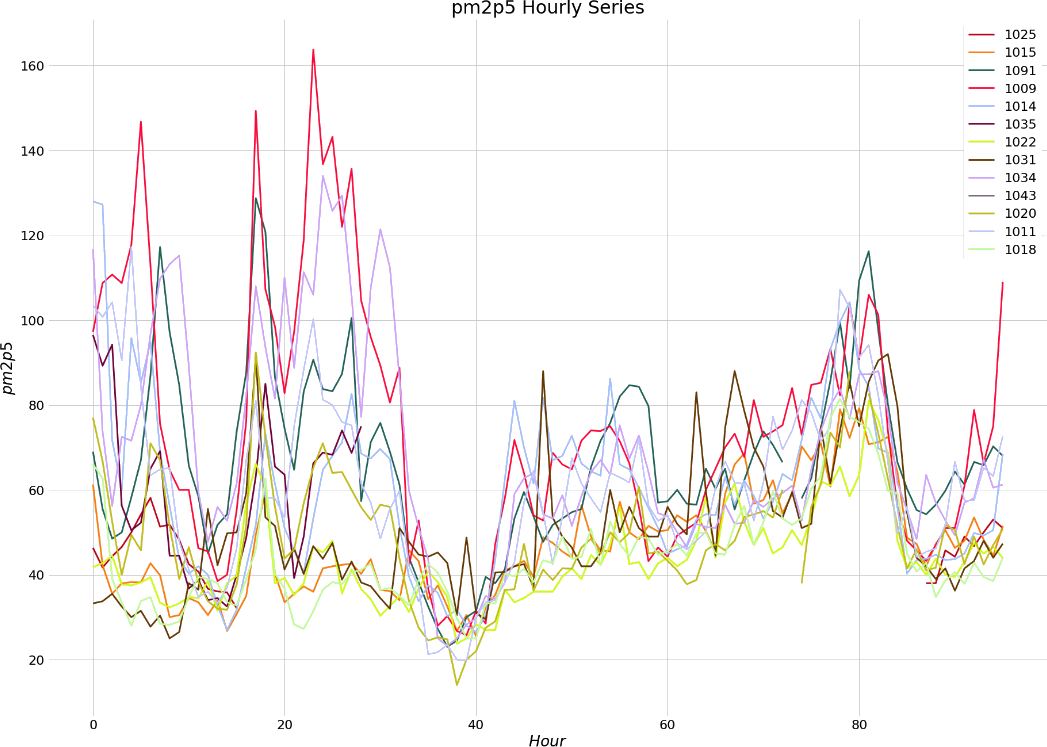
\includegraphics[scale=0.3]{plotDati.png}
    \caption{time series of pm2p5 in 48 hours for some pot-id}
\end{figure}
Wiseair own more than 60 air quality sensor in Milan at the moment and they are increasing day by day thanks to the involvement of citizens who install them. 

\\In our dataset they are identified by the variable potid. 
We consider only one potid to make some initial exploration, in particular we consider the \textbf{potid 1091} because it is the pot with less missing values.

 \begin{figure}[h!]
    \centering
    \begin{minipage}[t]{0.4\textwidth}
      \centering
      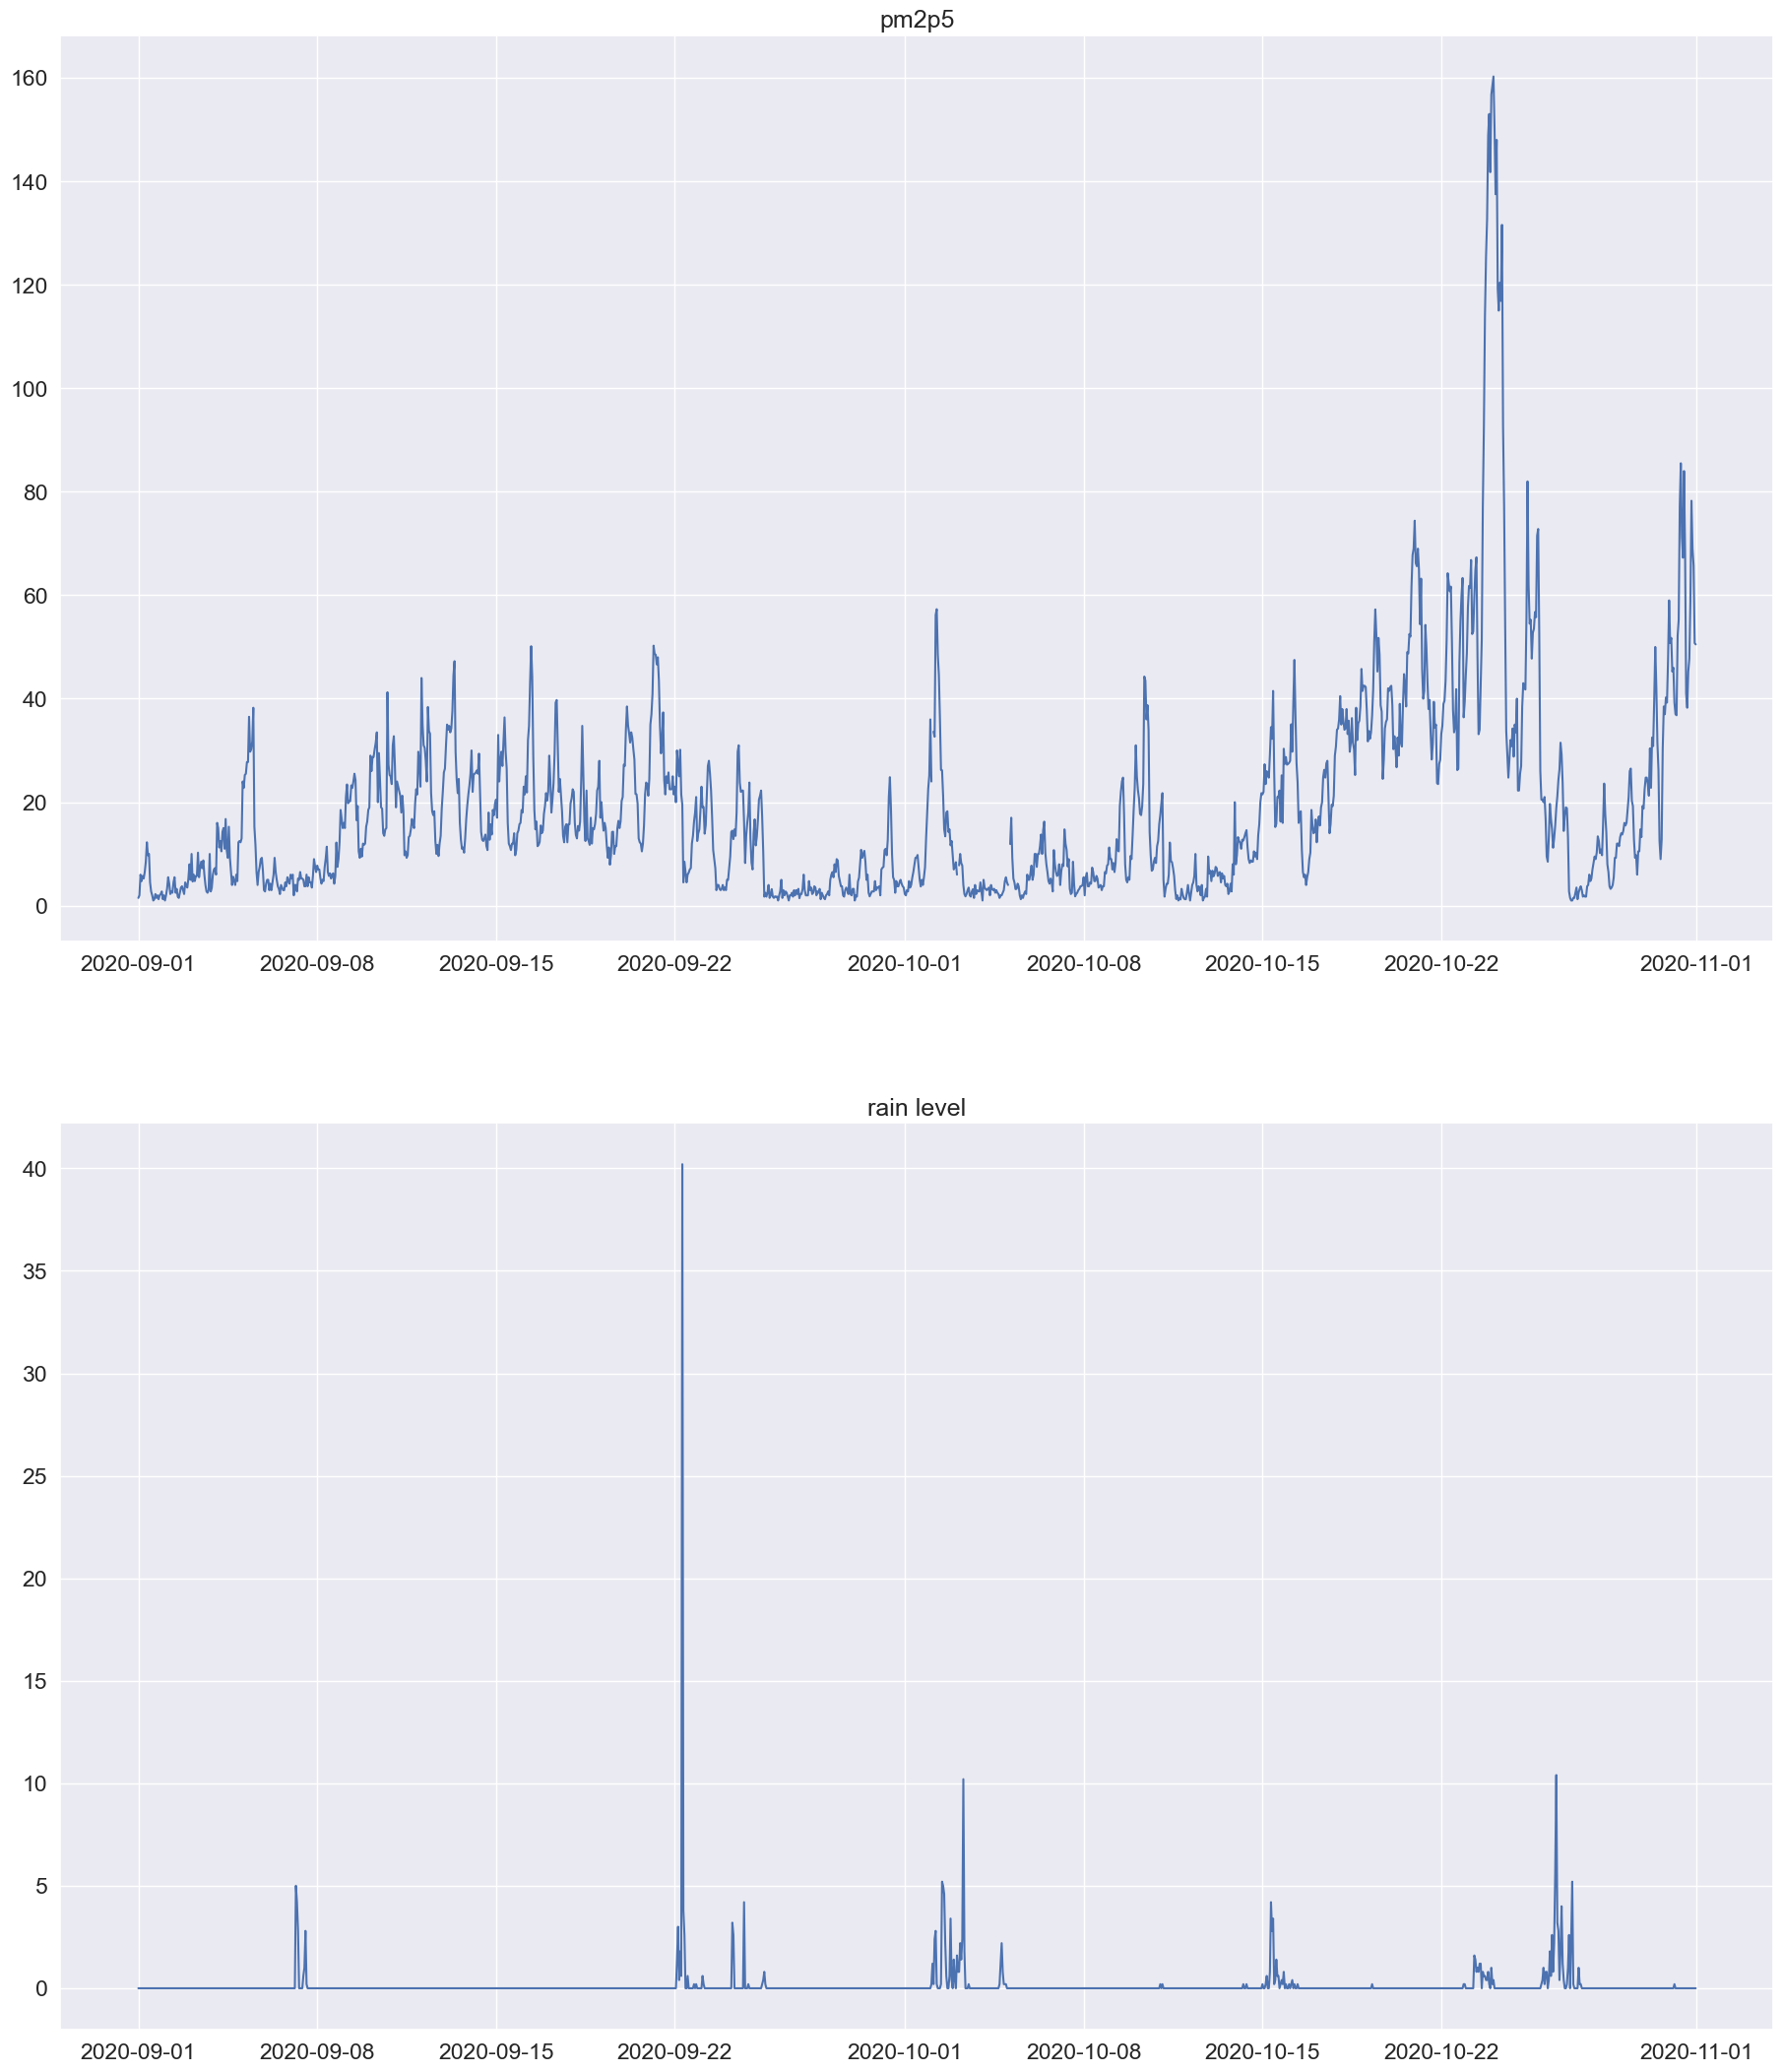
\includegraphics[scale=0.18]{plotpioggia.png}
      \caption{(a) Plot of rain vs pm2p5}
    \end{minipage}\hfill
    \begin{minipage}[t]{0.4\textwidth}
      \centering
      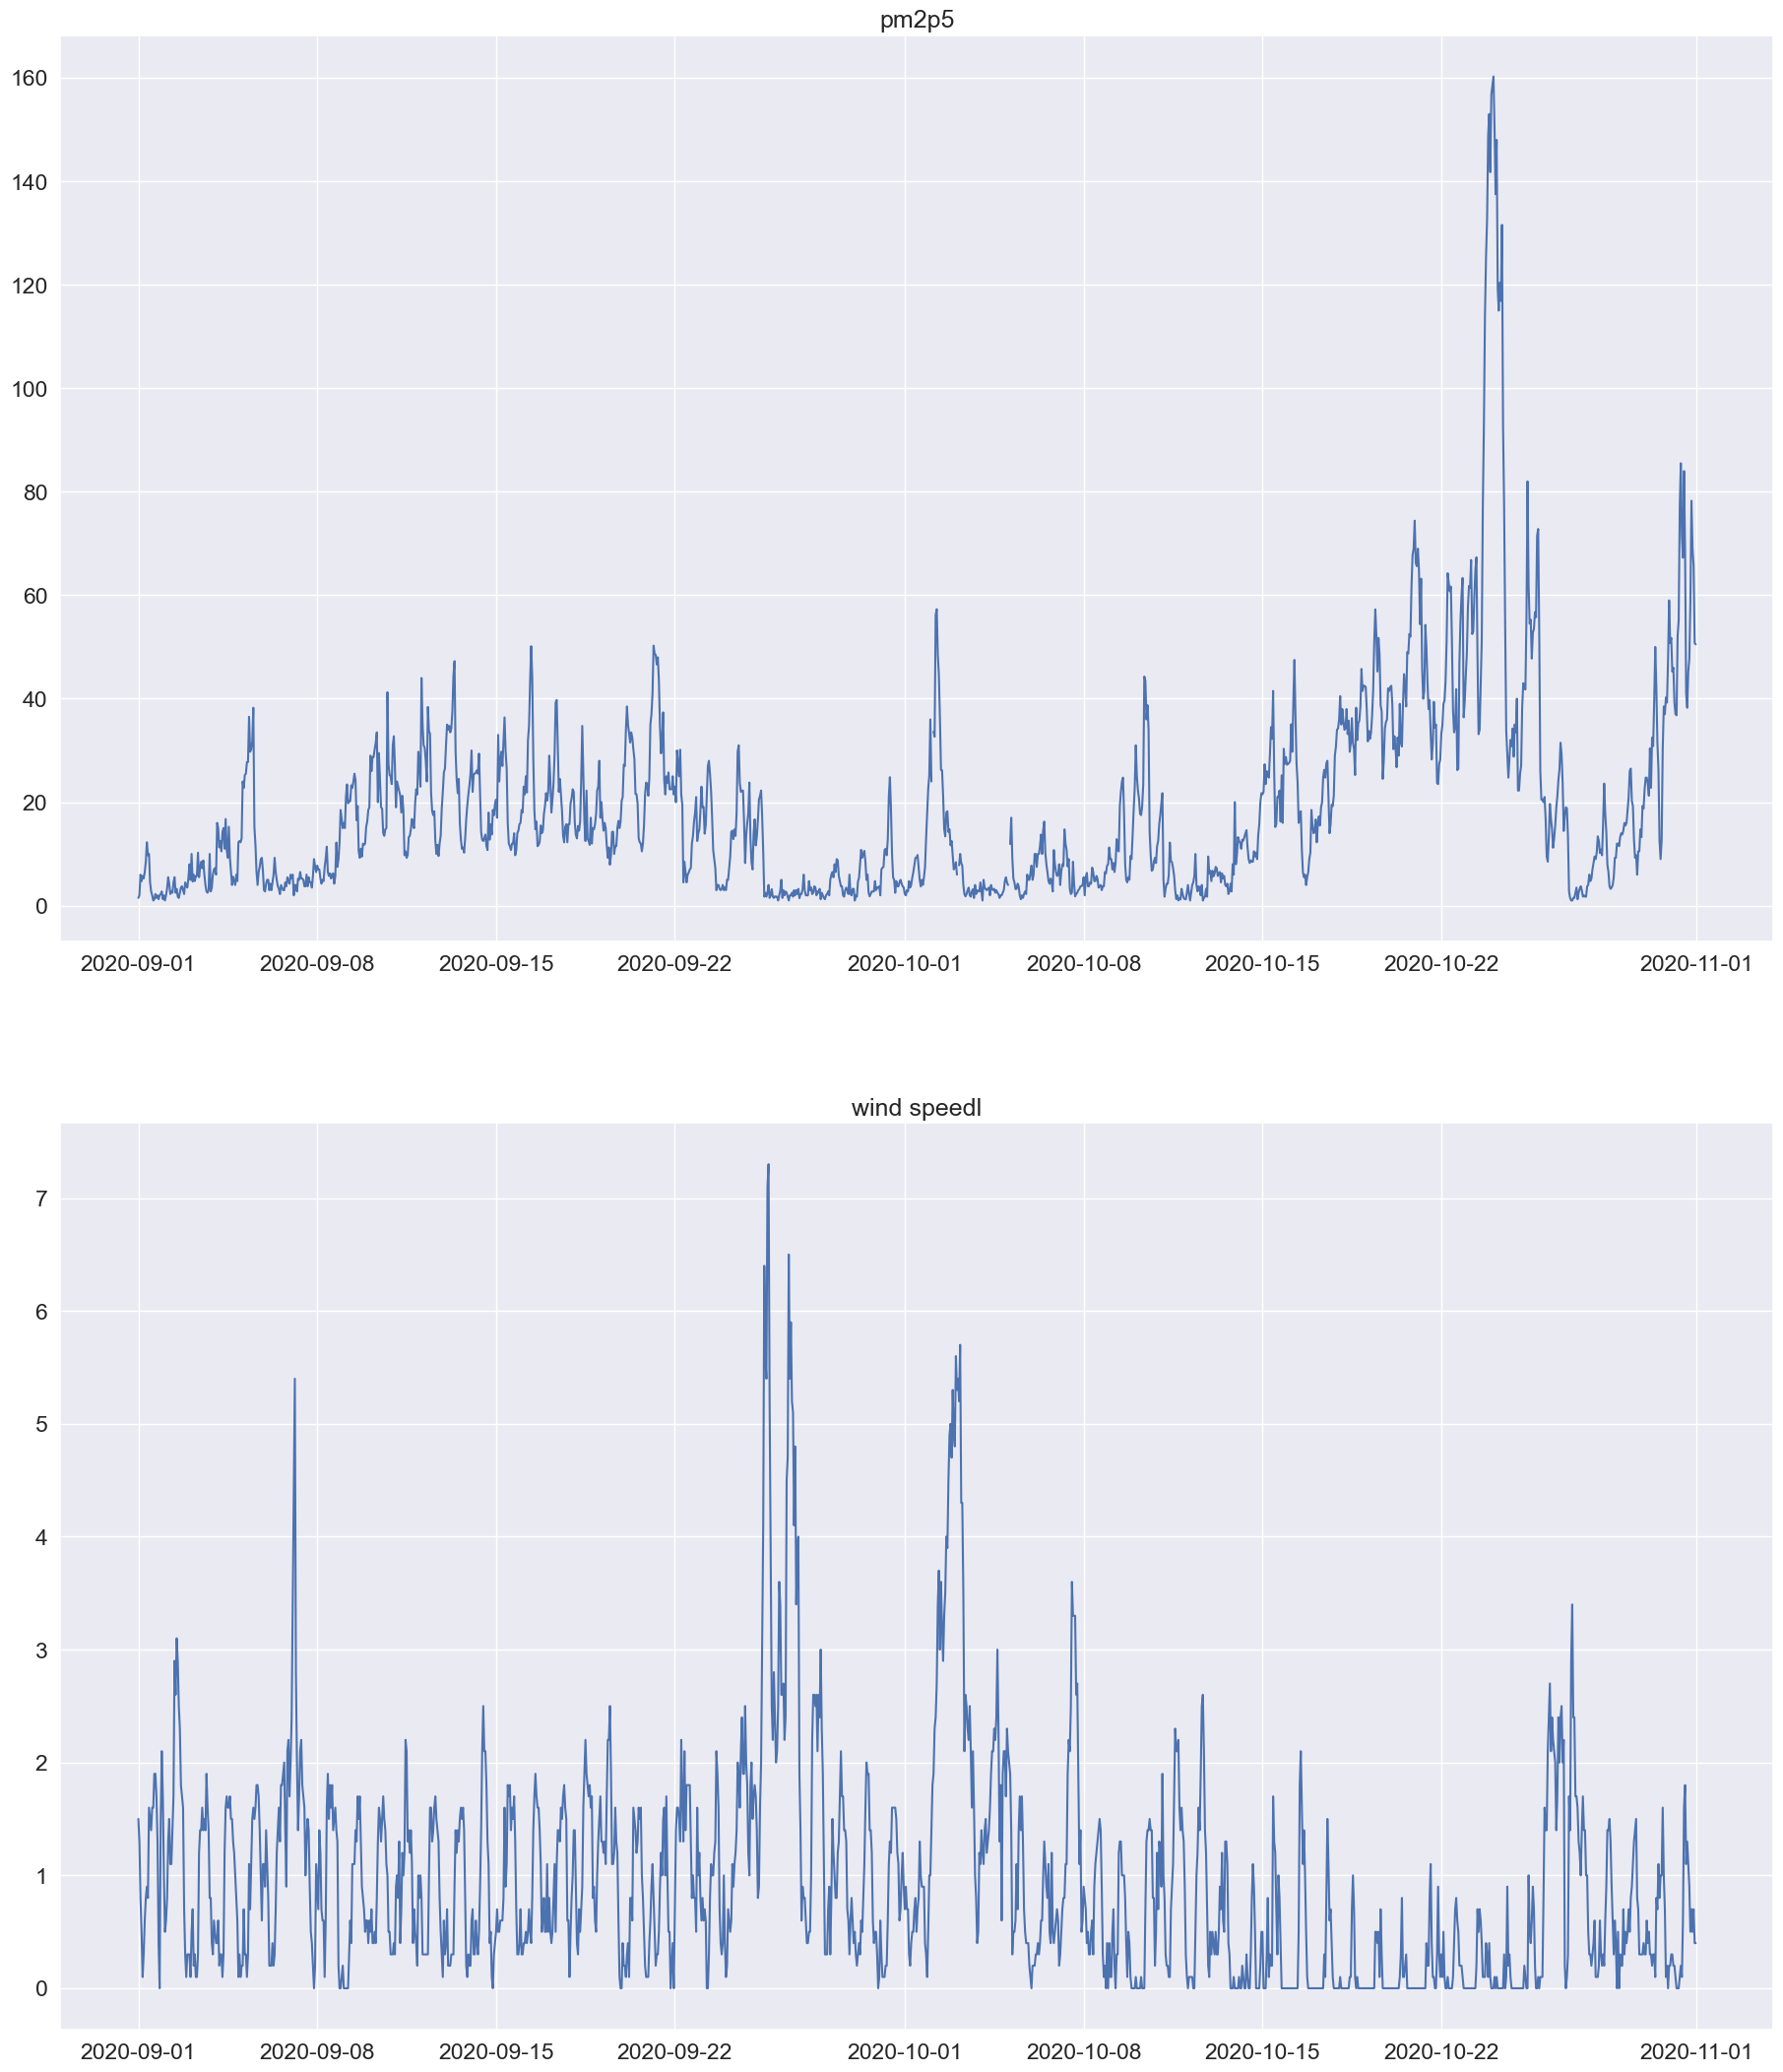
\includegraphics[scale=0.18]{plotwind.png}
      \caption{(b) Plot of wind speed vs pm2p5 }
    \end{minipage}
  \end{figure}
  
  \begin{figure}[h!]
    \centering
    \begin{minipage}[t]{0.4\textwidth}
      \centering
      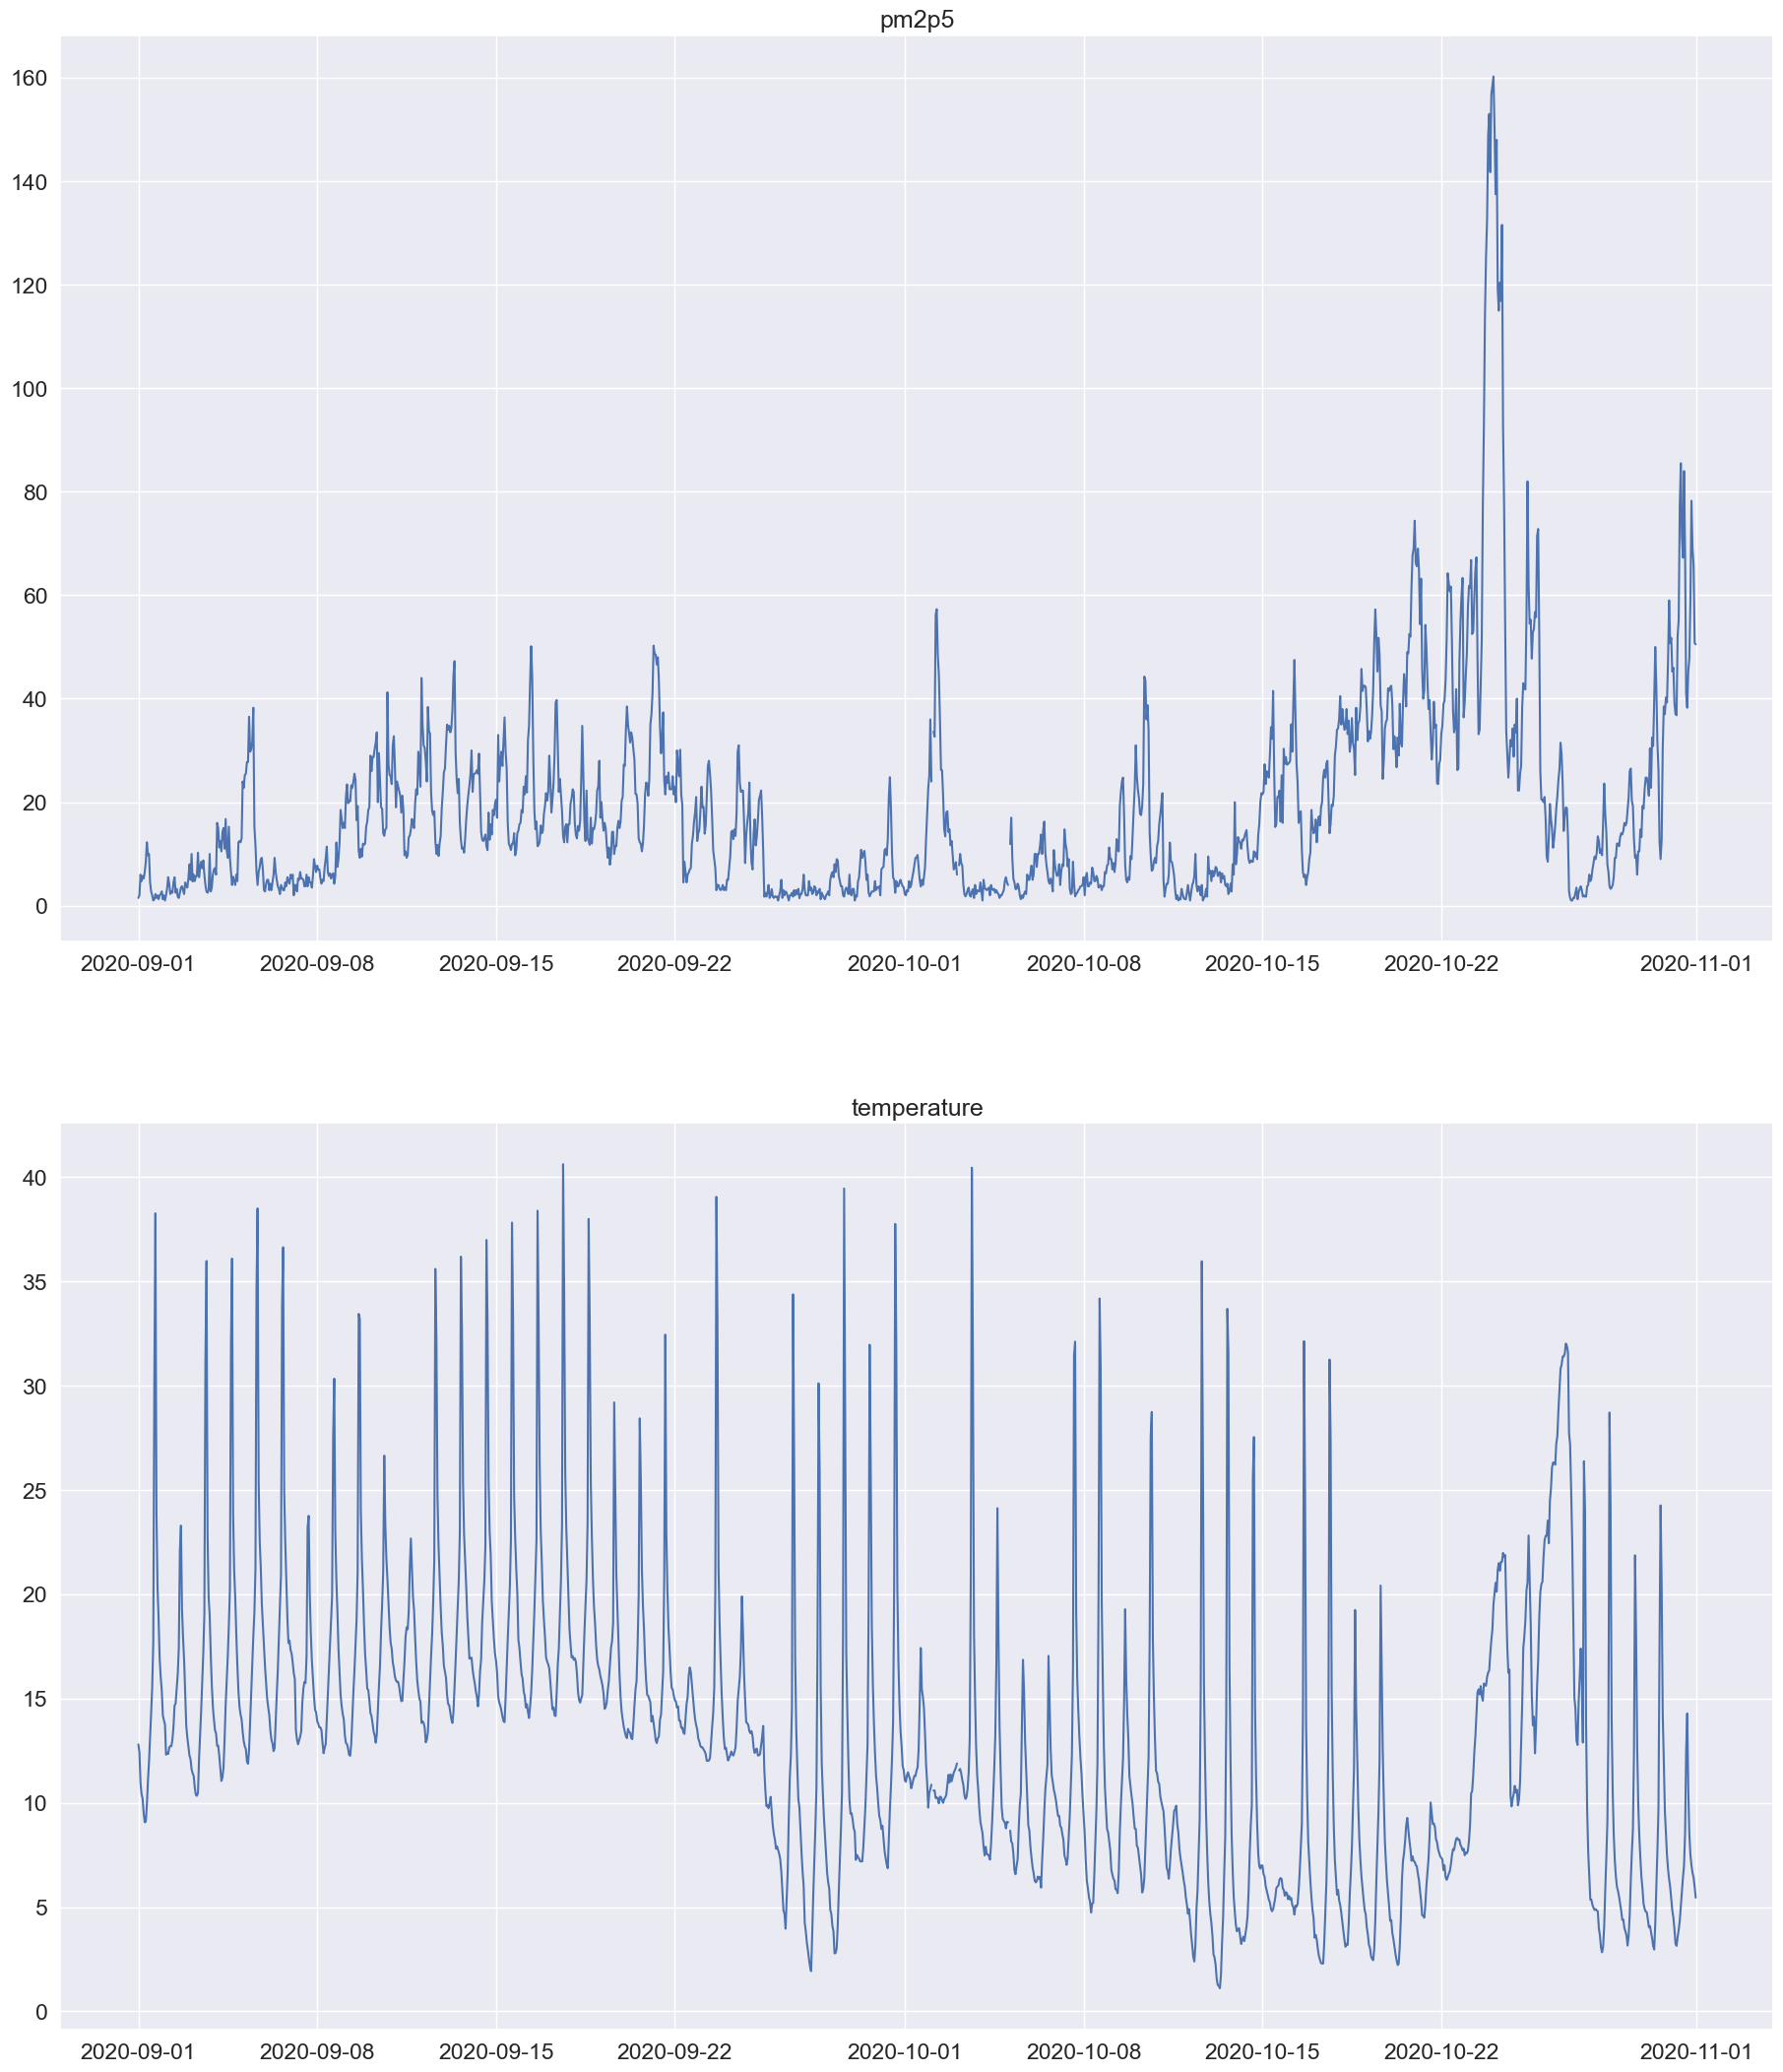
\includegraphics[scale=0.18]{plottemperature.png}
      \caption{(c) Plot of temperature vs pm2p5}
    \end{minipage}\hfill
    \begin{minipage}[t]{0.4\textwidth}
      \centering
      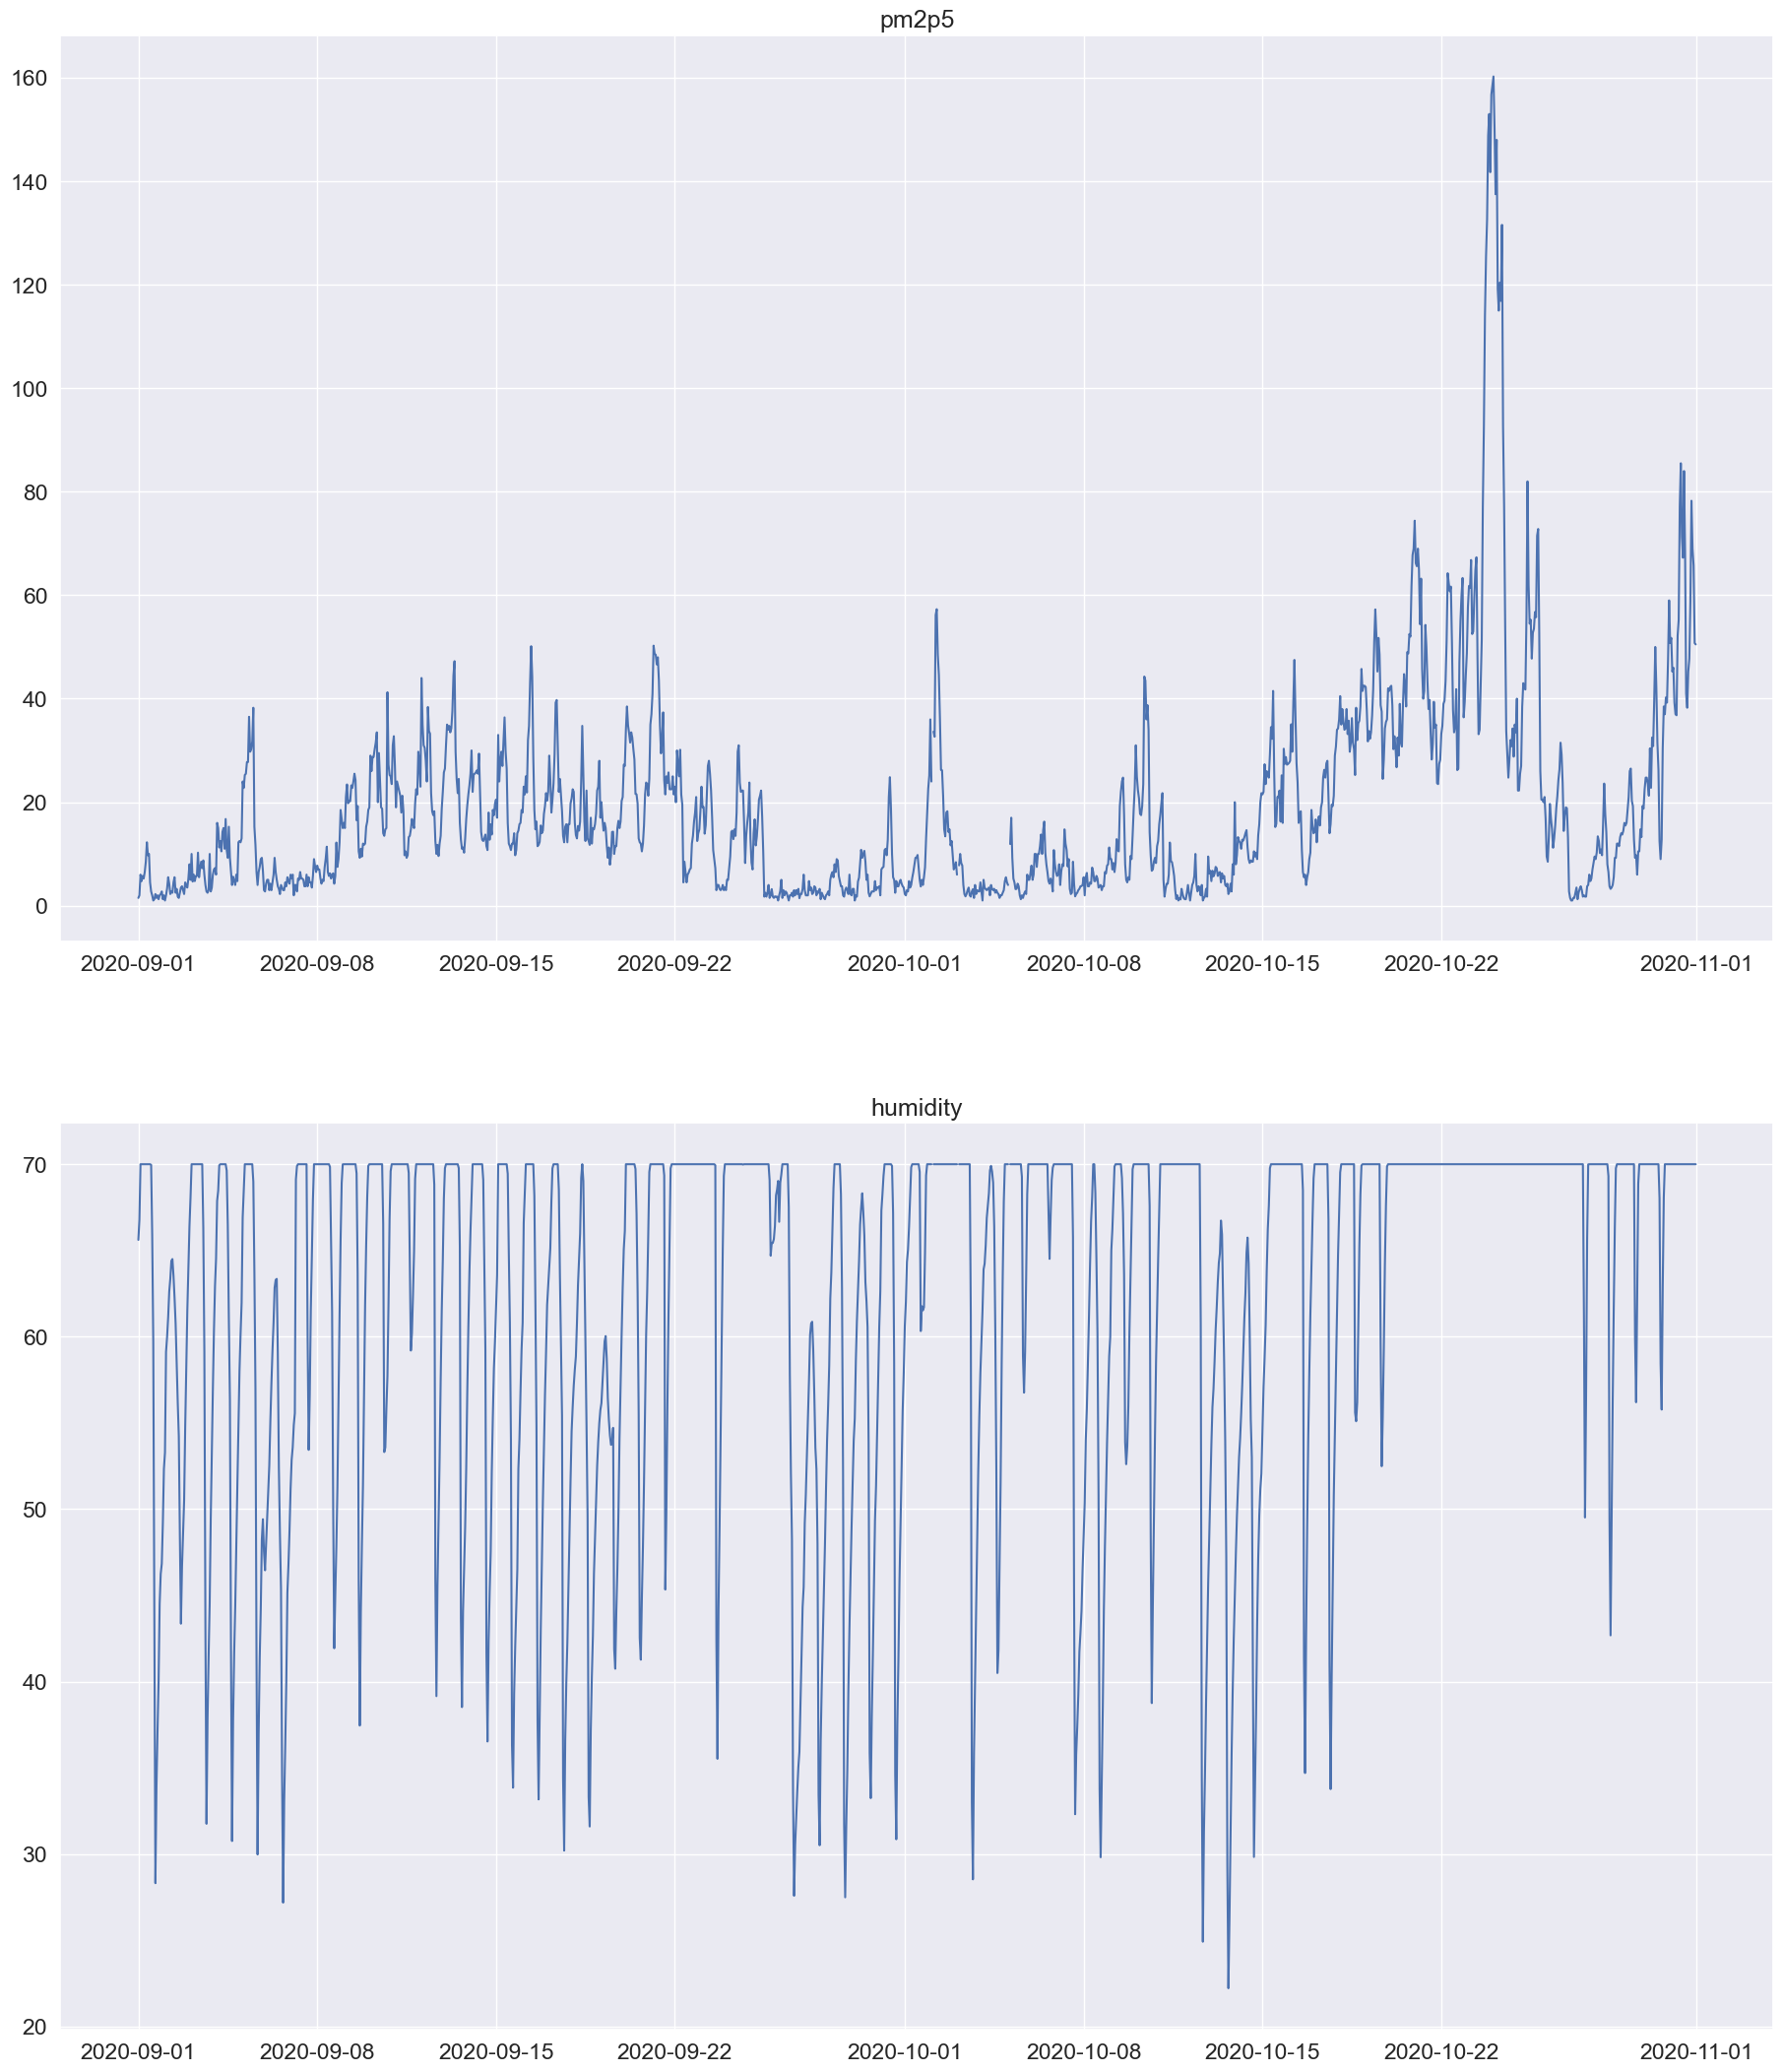
\includegraphics[scale=0.18]{humidityplot.png}
      \caption{(d) Plot of humidity vs pm2p5}
    \end{minipage}
  \end{figure}
The precision of sensors is negatively affected by special weather conditions (e.g.,
heavy rain, humidity, wind speed, temperature). Therefore, we examine atmospherical condition in order to find some interplay with the variation of pm2pm5.
 In the following graph, we show a qualitative comparison in the effect of rain, wind,humidity and temperature with the variation of pm2p5 in 48h for the potid 1091. 
 \\As for the moment just observe that there does not appear to be a strong relationship between
pm2p5 and rainy level or wind speed or temperature. A bit different is the nature of humidity. Even though the time series seems to
have a natural periodicity, the action of humidity sometimes disrupts this behaviour, since there is a big peak of pm2p5
in correspondence of a continuous high level of humidity(in the end of October).
\begin{wrapfigure}{r}{0.5\textwidth}
    \centering
    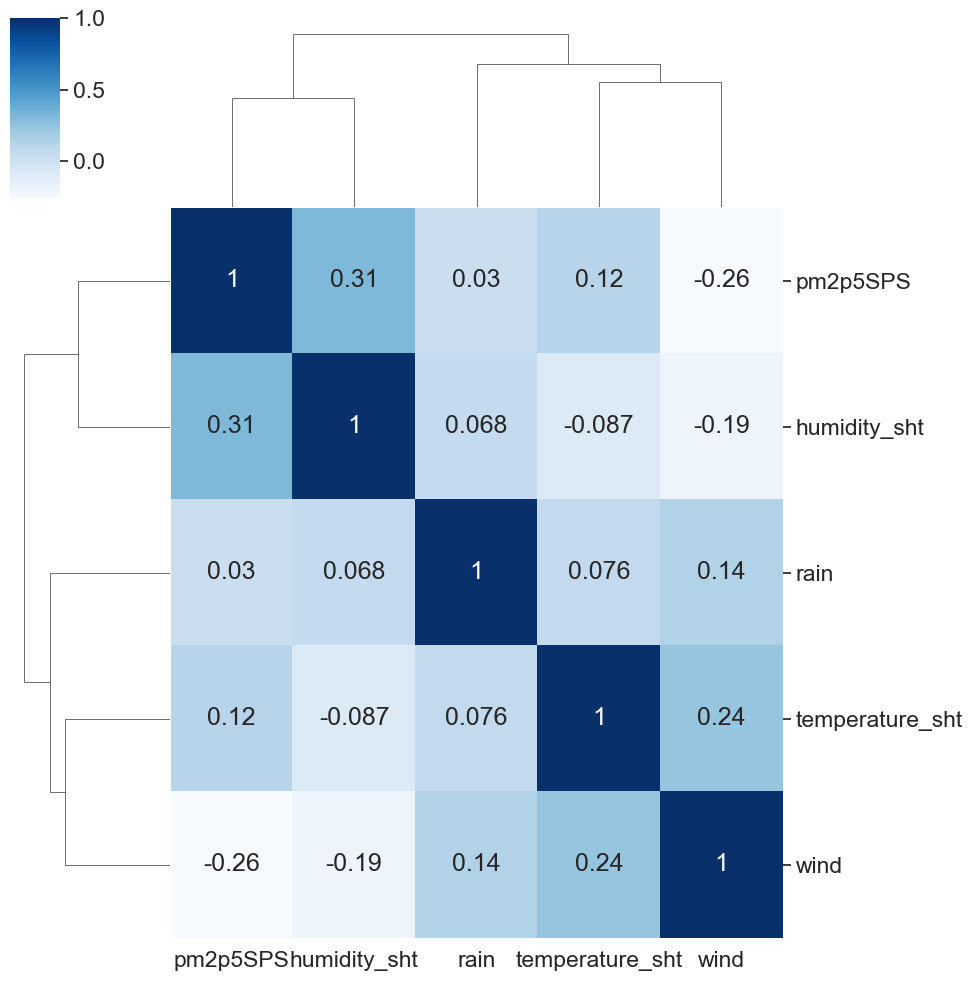
\includegraphics[scale=0.4]{correlations.png}
    \caption{clustermap}
\end{wrapfigure}

This can be seen also through the clustermap below, which plot a matrix dataset as a hierarchically-clustered heatmap . 
Motivated by these results, we will try to take into account this fact in our future analysis. 

\subsection{Stationarity}

In order to check the possibility to consider our model as a structural time series, we check the stationary of our time series such that its statistical properties (such as mean, variance, autocorrelation, etc.) are all constant over time. 
To check whether a series is stationary, we can apply the Augmented Dickey fuller test.
Since the p-value of the test is 0.020 we can reject the null hypothesis that the series is non-stationary. 

\section{Model}
Autoregressive time series models are central to stationary time series data analysis. Therefore, as  a first proposal, we choose an AR(2) model for the univariate case and we are going to extend this model with more complicated models for the multivariate case. We make this choice focusing on the analysis of the autocorrelation (ACF) and partial autocorrelation plot (PACF) of the pot 1091: 
since ACF tails off and PACF cuts off after one lag, then we are dealing with an AR(2) model (see figure~\ref{fig:acf} and~\ref{fig:pacf}).

  \begin{figure}[h!]
    \centering
    \begin{minipage}[t]{0.4\textwidth}
      \centering
      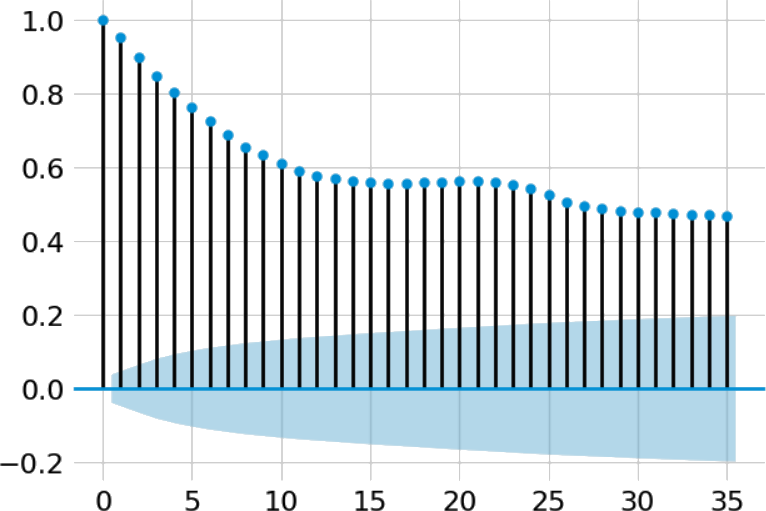
\includegraphics[scale=0.3]{acf.png}
      \caption{Autocorrelation plot for the 1091 pot series}\label{fig:acf}
    \end{minipage}\hfill
    \begin{minipage}[t]{0.4\textwidth}
      \centering
      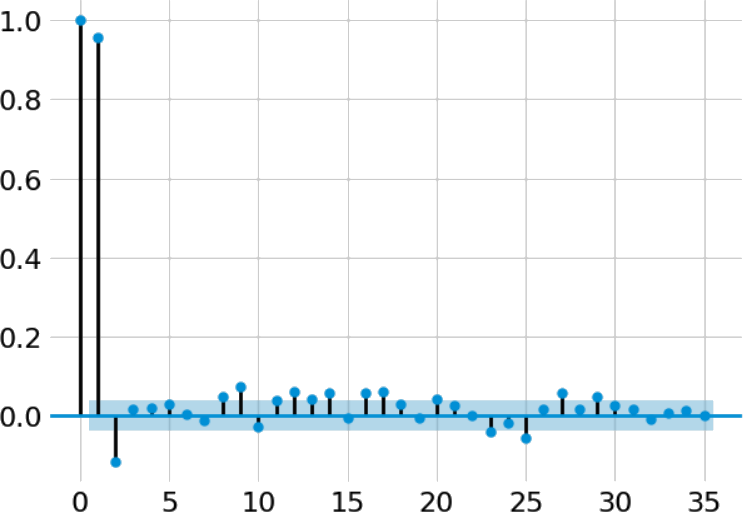
\includegraphics[scale=0.3]{pacf.png}
      \caption{Partial autocorrelation plot for the 1091 pot series}\label{fig:pacf}
    \end{minipage}
  \end{figure}

As a first proposal, we assume a conjugate model to explain the AR(2) structure of the time series:
\begin{equation*}
    y_t = \phi_1 y_{t-1} + \phi_2 y_{t-2} + \epsilon_{t} \qquad \qquad \epsilon_{t} \sim \mathcal{N}(0, \sigma^2) 
\end{equation*}
where $\epsilon_{t}$ is a sequence of uncorrelated error terms and the $\phi_i$ are constant parameters.

\vspace{3mm}
\begin{tabularx}{0.8\textwidth}{XX}
    {
        \text{LIKELIHOOD}\newline\newline
        \begin{aligned} 
        y|\underline{\phi},\beta & \sim N(\underline{\phi}^{T}\beta,\sigma^{2})\\
        & \text{$\sigma^{2}$ not known}
        \end{aligned}
    }&{
        \text{PRIORS}\newline\newline
        \begin{aligned}
	    \underline{\phi }|\sigma^2 &\sim \mathcal{N}_2(\underline\mu_0, \sigma^2B_0) \\
        \sigma^2 &\sim inv\Gamma \Bigl(\frac{\nu_0}{2}, \frac{\nu_0 \sigma_0^2}{2} \Bigr) \qquad
        \text{with $\mu_0, B_0, \nu_0, \sigma_0^2$ fixed}
        \end{aligned}
    }
\end{tabularx}
\vspace{3mm}

$B_0$ is a $2 \times 2$ matrix, $\mu_0$ is any vector in $\mathcal{R}^2$. Because the model is a standard conjugate linear model, posteriors are:

\text{POSTERIORS}\newline\newline
\begin{aligned}
\underline{\phi} | Y &\sim \mathcal{N}_2 (\mu_n, \sigma^2 B_n)
\qquad \qquad
\begin{aligned}
    & \mu_n = \mu_0 + B_0 \Phi[\Phi^{T} B_0 \Phi + I_n]^{-1}(Y - \Phi^T\mu_0) \\
    & B_n = B_0 - B_0\Phi[\Phi^{T} B_0 \Phi + I_n]^{-1}\Phi^T B_0 \\
\end{aligned} \\
\sigma^2 | Y &\sim inv\Gamma \Biggl(\frac{v_n}{2}, \frac{v_n \sigma_n^2}{2} \Biggr) 
\qquad \qquad 
\begin{aligned}
    & v_n = v_0 + n \\
    & \sigma_n^2 = \frac{1}{v_n} \Bigl[ v_0\sigma_0^2 + (Y - \Phi^T\mu_0)^T [\Phi^T B_0 \Phi + I_n]^{-1} (Y - \Phi^T\mu_0) \Bigr]
    \end{aligned}\\
\end{aligned}

\vspace{10mm}

Unfortunately can happen that sensor does not send any data. From our perspective this translates in the presence of missing values in the time series. For this univariate analysis pot 1091 has only the 0.012\% of value missing, hence in this case is not a particular problem. Morover missing data are distributed over the all considered period (we have missing values in correspondence of just few hours) and do not span a large interval of time.

\end{document}
